\clearpage

\section{Mechanics of structures}

The aim of this section is not to give a comprehensive grounding in structures, there are structural engineers for that sort of thing, but to at least look at the basics to see how material choices and structural design choices can be linked.

\subsection{Recap of bending moments and beam stiffness}

A moment, $M$, is generated by the application of a force (or forces) with some transverse separation. It is calculated by:
\begin{equation}
M = FL
\end{equation}
where $F$ is the component of the forces perpendicular to the separation $L$. Using this we can calculate how a moment varies along a cantilever loaded at one end and fixed at the other:

\FloatBarrier
\begin{figure}[h!]
\centering
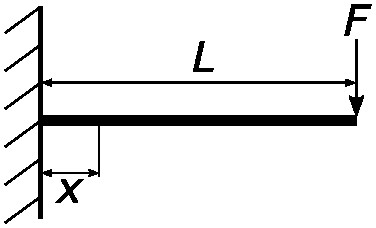
\includegraphics[width=0.5\textwidth]{end_loaded_cantilever}
\caption{A cantilever fixed at one end and loaded transversely at the other.\label{fig:simple_cantilever}}
\end{figure}
\FloatBarrier

This gives a moment at a position $x$ of:
\begin{equation}
\begin{annotation}
M=F(L-x)
\end{annotation}
\end{equation}
And this can be extended to multiple forces:
\FloatBarrier
\begin{figure}
\centering
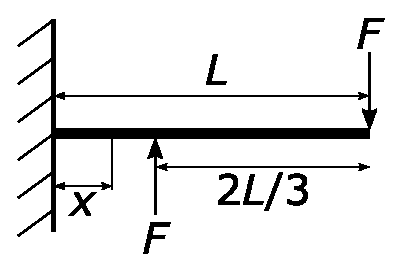
\includegraphics[width=0.5\textwidth]{two_forces_cantilever}
\caption{A cantilever with two applied forces.}
\end{figure}
\FloatBarrier
This gives the moment at the point $x$ as:
\begin{equation}
\begin{annotation}
M=F(L-x) - F(L/3 - x)
\end{annotation}
\end{equation}

This is then linked to the material by the beam stiffness equation:
\begin{equation}
M=\kappa EI \label{eqn:beam_bending}
\end{equation}
where $I$ is the second moment of area and is calculated by:
\begin{equation}
 I = \int_A y^2 dA 
\end{equation}
where $dA$ is an element of area at a distance $y$ from the neutral axis.

This can be applied even to complex arrangements of forces along beams or even distributed forces, as long as an expression for the moment at any point is obtainable.

We can find the deflection of a point along the beam by approximating the second derivative of the height of the beam as equal to the curvature:
\FloatBarrier
\begin{figure}[h!]
\centering
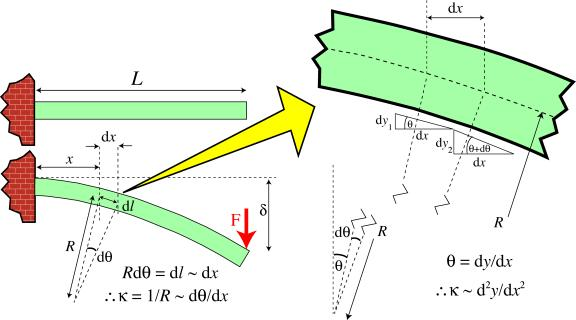
\includegraphics[width=\textwidth]{moment_diagram1}
\caption{The approximation, valid for small deflections, that the curvature of the beam and of the neutral axis are equal. Reproduced from \cite{doitpoms_beams}.}
\end{figure}
\FloatBarrier

This gives us:
\begin{equation}
\kappa = \frac{d^2y}{dx^2}
\end{equation}

and we can substitute this into the beam bending equation (\autoref{eqn:beam_bending}):
\begin{equation}
\frac{d^2y}{dx^2}=\kappa = \frac{M}{EI} \label{eqn:beam_curvature}
\end{equation}

Using this we can use the balance of moments between the internal moments and external moments to find an expression for the shape of the deformed beam.

Considering the end loaded cantilever above we can write:
\begin{equation}
EI \frac{d^2y}{dx^2} = M = F(L-x)
\end{equation}
where $x$ is as defined in \autoref{fig:simple_cantilever}. This can be integrated:
\begin{equation}
EI\frac{dy}{dx} = FLx - \frac{Fx^2}{2} + c_1
\end{equation}
Since at the wall, $x=0$ and $\frac{dy}{dx} = 0$, the constant $C_1=0$. We can then integrate again:
\begin{equation}
EIy = \frac{FLx^2}{2} - \frac{Fx^3}{6} + C_2
\end{equation}
Again, the boundary condition that at $x=0$, $y=0$ so therefore $C_2=0$, giving the final expression:
\begin{equation}
y = \frac{Fx^2}{6EI}(3L-x)
\end{equation}
and therefore the maximum deflection is
\begin{equation}
\delta = \frac{FL^3}{3EI} \qquad \begin{annotation}\text{and this occurs at} \,\, x=L
\end{annotation}
\end{equation}


Problems of this type are all solved in this manner, balancing the moments de to the internal stresses and an externally applied moment. There are two main challenges, the first is to find an expression for the external moment, which can be complex if there is more than one force applied. This expression can and will vary along the length of the beam, changing as the reference point passes the position of applied forces.

The second key point is to identify the boundary conditions, which usually rely on known fixed points where the displacement, or the gradient must be zero, or that the beams displacement and gradient must be continuous.









\subsubsection{The parallel axis theorem}


This can be adjusted to be about another parallel axis displaced by a distance $d$ form the neutral axis:
\begin{equation}
I_{\text{parallel}} = \int_A (y+d)^2dA = \int y^2 dA + 2 d \int y dA + d^2\int dA
\end{equation}

Since the distance $y$ is to the neutral axis, the second term must be zero (the neutral axis passes through the centre of mass). This leaves what is know as the parallel axis theorem:
\begin{equation}
I_{\text{parallel}} = I_{\text{neutral}} + d^2A
\end{equation}

\subsubsection{Stresses and strains in a beam}

To recap from IA, the strains in a bent beam can be found straight forwardly from the diagram in \autoref{fig:strain_from_curvature}.
\FloatBarrier
\begin{figure}[h!]
\centering
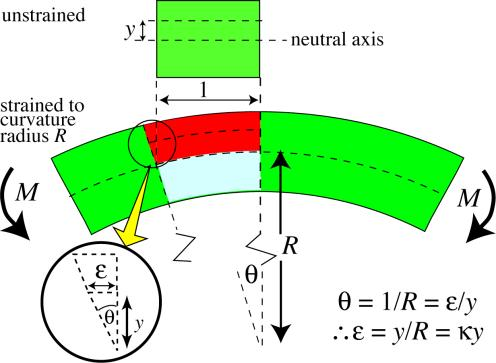
\includegraphics[width=0.5\textwidth]{bend_diagram2}
\caption{The relationship between curvature and strain in a bent beam. Reproduced from the DoITPoMS TLP \cite{doitpoms_beams}.\label{fig:strain_from_curvature}}
\end{figure}
\FloatBarrier

If we assume that the deformation remains elastic then we can relate the strain to the stress simply by: $\sigma = E \varepsilon = E\kappa y$

This can be used to derive the beam bending equation:

\FloatBarrier
\begin{figure}[h!]
\centering
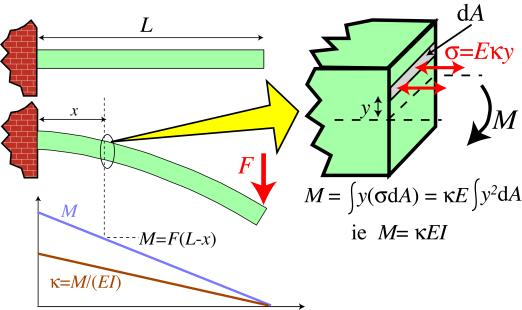
\includegraphics[width=0.8\textwidth]{bend_diagram}
\caption{The balance between the externally applied moments and the internally generated moments due to stresses.\label{}}
\end{figure}
\FloatBarrier

\subsubsection{Torsion}

Torsion is the application of a {\bf torque (twisting moment)} to induce a {\bf twist} in a beam. Torques are common in engineering situations, for example in service for shafts in engines and bridges, but also in construction in screws and bolts. They can also arise is more unexpected places such as boat hulls or aeroplane fuselages. 

A torque (usually denoted $T$) has the same units (\si{\newton\meter}) as bending moments (usually $M$), as both are a product of a force and a perpendicular distance. The difference is in their orientation relative to the beam. Bending moments are parallel to the radius (of a round beam), and act through the beam; a torque is a tangential force that is offset radially from the axis of rotation.

Torsion is simple for thin walled cylinders where the stress cannot vary much across the thickness of the wall, the problem becomes one of simple force balance:


\FloatBarrier
\begin{figure}[h!]
\centering
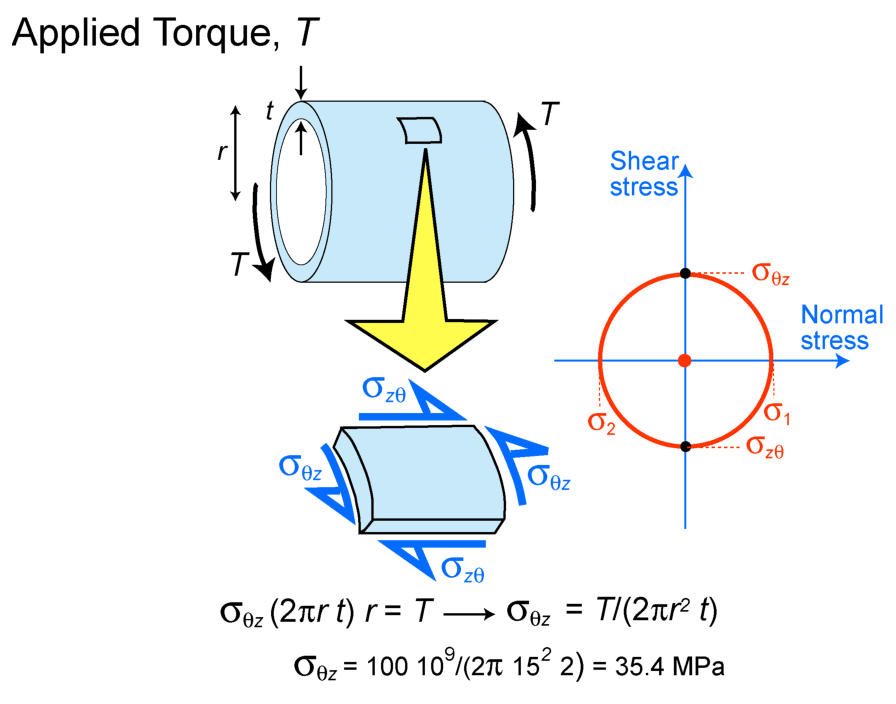
\includegraphics[width=0.6\textwidth]{thin_wall_torsion}
\caption{Stresses that arise due to a torsion applied to a thin walled cylinder. Mohr's Circle can be used to find the principal stesses.}
\end{figure}
\FloatBarrier
The result is:
\begin{align}
T= \sigma_{\theta z} (2\pi r t) r \nonumber \\
\implies \sigma_{\theta z} = \frac{T}{2 \pi r^2 t}
\end{align}


It is important to remember the assumptions that have been made in reaching this point (in fact it's always important). In this case the assumption relies on the wall being thin and therefore that the stresses do not vary significantly across the thickness of the wall. This is not the case for a solid cylindrical shaft or thick walled cylinders.

Since solid cylinders are more usual for transferring torque (e.g.\ drive shafts). In this case the stress will vary with the radial position.

\FloatBarrier
\begin{figure}[h!]
\centering
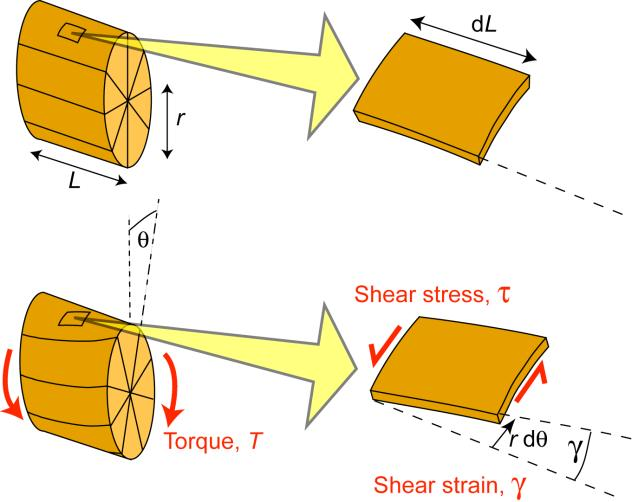
\includegraphics[width=0.55\textwidth]{twist_diagram}
\caption{The application of a torque to a solid cylinder and the development of shear strains.}
\end{figure}
\FloatBarrier


By considering a straight reference line along the axis of the shaft being displaced we can define the strain:

\FloatBarrier
\begin{figure}[h!]
\centering
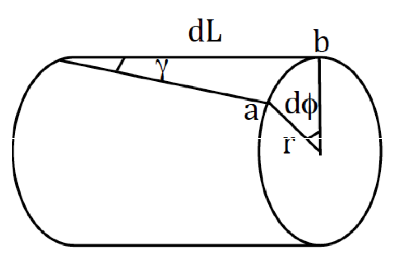
\includegraphics[width=0.3\textwidth]{torsional_strain}
\end{figure}
\FloatBarrier

The strain (the $\theta z$ component) is given by:
\begin{equation}
\begin{annotation}
\gamma_{\theta z} = d\frac{d\phi}{dL}
\end{annotation}
\end{equation}

Which we can relate to the overall twist in the bar to find the maximum shear strain (which will occur at the outside of the bar):
\begin{equation}
\gamma_{\theta z}^{\text{max}} = \frac{R\phi}{L}
\end{equation}
Assuming that the rate of twist can be calculated from the total angle of twist, $\phi$, and the total length of bar, $L$.

This can be converted to a stress by assuming that Hooke's Law holds (i.e.\ $\sigma_{\theta z} = G \gamma_{\theta z}$):
\begin{equation}
\sigma_{\theta z} = G r \frac{d\phi}{dL}
\end{equation}


We now have a handle on the force balance that must arise in equilibrium, i.e.\ the internal stresses must balance the external torque:

\begin{equation}
T = \int dT = \int \sigma_{\theta z} r dA = \int Gr^2 \frac{d\phi}{dL}dA
\end{equation}

By analogy with beam bending there is a geometric term which is the {\bf polar} second moment of area:
\begin{equation}
I_{\text{P}} = \int r^2 dA
\end{equation}
and there is also an expression equivalent to the beam bending equation ($M=EI\kappa$):
\begin{equation}
T = G I_{\text{P}} \frac{d\phi}{dL}
\end{equation}
where the rate of twist is the equivalent to the curvature of a cantilever.

%% NB a question on this might be to find the maximum stress for the drive shaft of a car engine (maybe even consider the weight/cost)
























































\clearpage